\section{化学热力学}
\subsection{热力学的基本概念}
\begin{definition}[热力学系统]
热力学系统是指选定用于实验或理论研究的特定部分。系统之外一切其余部分定义为环境，而宇宙则是系统与环境的总和。
\end{definition}

根据系统与环境之间的物质和能量交换，可将系统分为以下几类：
\begin{enumerate}
    \item 敞开系统：与环境同时交换物质和能量；
    \item 封闭系统：与环境交换能量但不交换物质；
    \item 孤立系统：与环境既不交换物质也不交换能量。
\end{enumerate}

若描述系统的所有宏观物理性质都具有唯一确定的值，则称该系统处于确定的状态状态函数是指变化仅取决于系统的始态和终态，而与变化途径无关的物理量（例如 $V$、$T$、$p$）。

广延量是对各子系统具有加和性的状态函数（例如体积 $V$、物质的量 $n$、内能 $U$）。强度量是不具有加和性且与系统大小无关的状态函数，通常为两个广延量的比值（例如压力 $p$、温度 $T$、密度 $\rho$）。

过程量为非状态函数，其变化取决于系统状态变化的途径。

确定研究的系统后，我们可以像分析力学那样从能量的角度考虑其与环境的相互作用。我们将系统或环境的总能量称为热力学能（$U$），也称为内能，其绝对量不可知。

当两个系统处于热接触状态时，若它们之间没有净的能量传递，则称这两个系统处于热平衡状态。

\begin{proposition}[热力学第零定律]
若两个系统分别与第三个系统处于热平衡，则这两个系统彼此也处于热平衡。换句话说，这定义划分了一个等价类。
\end{proposition}
由于热平衡是等价关系，我们可以为每个等价类分配唯一的数值，这个数值就是我们所说的 温度（$T$）。

基于温度，系统与环境之间的相互作用可分为两类：一类由温度差引起，我们称之为热（$Q$），其余部分则为功（$W$）。显然，它们都不是状态函数。


绝热过程被定义为允许功但是不允许热的过程。

\begin{proposition}[热力学第一定律]
封闭系统的内能变化等于外界对系统所做的功与系统吸收的热之和，核心公式为：$$\Delta U = U_f - U_i = W + Q$$ 
其微分形式为：（注：d 仅用于状态函数，$\delta$仅为无穷小量的标记）
$$dU = \delta W +\delta Q $$
其中 $\Delta U$ 为内能变化，$U_f$ 和 $U_i$ 分别为系统的终态和始态内能。$W$ 为功，$Q$ 为热，符号上，系统获得能量时，$W$ 和 $Q$ 取正值；系统失去能量时，取负值。
\end{proposition}

对于宇宙而言，不存在环境，此时：
$$W=Q=0$$ 
即 $U$ 为常数，换句话说，宇宙的能量是守恒的。

接下来我们可以分别研究功和热。

最重要的一类功是体积功（$W_e$），也称为膨胀功，其定义为系统因体积变化对抗外压所做的功（或外界对系统做的功），遵循力学中功的基本定义 $\delta W=F dr$。注意到力和压强、体积和位矢之间的关系：
$$F = - p S, \quad dV = S dr$$ 
可得：

\begin{proposition}[体积功]
$$\delta W_e = -p_{ex}dV, \quad W_e = \int_{V_1}^{V_2} -p_{ex}dV$$
其中 $p_{ex}$ 为外压，$dV$ 为系统的体积无穷小变化。对于理想气体，典型可逆过程的体积功为：
\begin{enumerate}
    \item 恒压过程（$p_{ex}=\text{常数}$）：$W_e = -p(V_2 - V_1)$；
    \item 恒温过程（$T=\text{常数}$）：$W_e = - \nu RT\ln\frac{V_2}{V_1}$；
    \item 恒容过程（$V=\text{常数}$）：$W_e = 0$。
\end{enumerate}
\end{proposition}

我们将其余的所有功称为非体积功（$W_f$），将在后续章节中研究。本章中假设不存在非体积功。

首先是关于恒容状态的，在这种情况下$W = W_e + W_f = 0$，结合热一律，$\Delta U = Q + W = Q$，我们用记号$Q_V$来指示恒容状态:

\begin{definition}[恒容（反应）热]
对于仅存在体积功（$W_f=0$）的封闭系统，其在恒容条件下吸收或放出的热（$Q_V$）称为恒容热，其大小等于系统的内能变：$Q_V = \Delta U$。
\end{definition}

对于恒压过程，我们对体积功的计算，给出了$\Delta U = U_f - U_i = W + Q =Q - p_{ex} (V_f - V_i )$，整理得：$$Q =(U_f + p_{ex} V_f ) - (U_i + p_{ex} V_i)$$我们发现量$U + p V$指示了热，于是定义：

\begin{definition}[焓（恒压（反应）热）]
焓（$H$）是定义为 $H = U + pV$ 的状态函数，其状态函数的性质由Hess（盖斯）定律指出。显然，其绝对量也不可知。

对于仅存在体积功（$W_f=0$）的封闭系统，其在恒压条件下吸收或放出的热（$Q_p$）称为恒压热，其大小等于系统的焓变：$Q_p = \Delta H$。
\end{definition}

\begin{proposition}[焓变与内能变化的关系]
对于涉及气体的反应，焓变与内能变化的关系为：
$$\Delta H = \Delta U + \Delta \nu_g RT$$
其中 $\Delta \nu_g = \sum \nu(\text{气体产物}) - \sum \nu(\text{气体反应物})$ 为反应前后气态物质的物质的量变化。
\end{proposition}

绝大多数的化学反应体系都是恒压的，所以我们着重讨论焓。由于焓的绝对量不可知，我们定义一个标准：

\begin{definition}[标准摩尔生成焓、燃烧焓与键焓]
\begin{enumerate}
    \item 标准摩尔生成焓（$\Delta_f H_m^\circ$）：在指定温度（通常为298.15 K）下，由最稳定的单质在标准状态下生成1摩尔纯物质时的焓变。
    \item 标准摩尔燃烧焓（$\Delta_c H_m^\circ$）：在指定温度下，1摩尔纯物质完全燃烧生成标准状态下的稳定氧化物时的焓变。
    \item 键焓（键解离能）（$BDE$）：在指定温度下，1摩尔某化学键断键的焓变。
\end{enumerate}
\end{definition}

从定义可以看出，焓是温度的函数，由于热容变化贡献（$\int C_p \,dT$）。当然，这不在普化的讨论范围。

在这些式子中，我们引入大量的角标，$\Delta$的角标代表对变化过程的描述，例如$f$为生成、$r$为反应等等；函数的角标$m$代表“每摩尔”，更准确来说是偏摩尔量，$H_{m,i} = \left( \frac{\partial H}{\partial n_i} \right)_{T, p, n_j (j \neq i)}$；而上标$^\circ$为标准状态，$p_i = 1 \text{bar}$，$c_i = 1 \text{M} $。

结合Hess定律，我们很容易给出：

\begin{proposition}[化学反应的焓变]
化学反应的标准偏摩尔焓变可通过以下公式计算：
$$\Delta_r H_m^\circ = \sum \nu \Delta_f H_m^\circ(\text{产物}) - \sum \nu \Delta_f H_m^\circ(\text{反应物})$$
$$\Delta_r H_m^\circ = \sum \nu \Delta_c H_m^\circ(\text{反应物}) - \sum \nu \Delta_c H_m^\circ(\text{产物})$$
也可通过键解离能估算：$\Delta_r H_m = \sum BDE(\text{反应物}) - \sum BDE(\text{产物})$
\end{proposition}

\subsection{化学反应的自发性}

热机是将热能转化为功的装置，Carnot（卡诺）热机是典型的热机，其由两个等温过程和两个绝热可逆过程组成的可逆循环，工作在高温热源$T_h$和低温热源$T_c$之间。热力学给出了：

\begin{proposition}[Carnot定理]
$$\eta = \frac{W}{Q_{in}} \leq 1 - \frac{T_c}{T_h}$$
其中$Q_{in}$ 为从高温热源吸收的热，$W$ 为热机对外做的功。
\end{proposition}

结合能量守恒 $Q_{in} = W + Q_{ex}$（$Q_{ex}$ 为向低温热源放出的热），可得：
$$\frac{-Q_{ex}}{T_c} + \frac{Q_{in}}{T_h} \geq 0$$


\begin{definition}[熵]
熵（$S$）是描述系统混乱度的状态函数，其可逆过程的微分定义为：
$$dS = \frac{\delta Q_{rev}}{T}$$
\end{definition}

带入即给出了$dS_{total} = dS_{sur} + dS_{sys} \geq 0$， 即：

\begin{proposition}[熵增原理（热力学第二定律等价表述）]
对于孤立系统，自发过程中熵永不减少：
$$\Delta S \geq 0$$
其中可逆过程 $\Delta S = 0$，不可逆过程 $\Delta S > 0$。
\end{proposition}

对于非孤立恒压系统，我们开始推导其自发性条件，$dS_{total} = dS_{sur} + dS_{sys}$，我们认为环境为可逆，带入熵的定义与热一律，整理得：

$$T dS_{total} = \delta W - dU + T dS_{sys} \geq 0 $$

结合体积功与焓的定义，给出：

$$dH - T dS_{sys} \leqslant 0 $$

\begin{definition}[Gibbs自由能（Gibbs-Helmholtz方程）]
Gibbs（吉布斯）自由能（$G$）是定义为 $G = H - TS$ 的状态函数，其中 $H$ 为焓，$T$ 为热力学温度，$S$ 为熵。对于恒温恒压无非体积功的过程，热力学自发性判据为：
$$dG < 0 \ (\text{自发过程}),\quad \ dG = 0 \ (\text{平衡状态}),\quad \ dG > 0 \ (\text{非自发过程})$$
当然，这是热力学上的，并不代表一定（收到动力学限制）。
\end{definition}

当然，涉及非体积功时：

\begin{proposition}[热力学允许条件]
$$\Delta_r G_m < W_f$$
从这里可以看出，Gibbs自由能衡量了体系对外做非体积功的能力。
\end{proposition}



从气体出发并推广，van't Hoff(范特霍夫)给出了偏摩尔Gibbs自由能随浓度（反应商）变化的方程：

\begin{definition}[浓度商]
对于一般反应 $aA + bB \rightleftharpoons cC + dD$，反应商为：
$$Q_c = \frac{\left(\frac{[C]}{c^\circ}\right)^c \left(\frac{[D]}{c^\circ}\right)^d}{\left(\frac{[A]}{c^\circ}\right)^a \left(\frac{[B]}{c^\circ}\right)^b},\quad Q_p = \frac{\left(\frac{[C]}{p^\circ}\right)^c \left(\frac{[D]}{p^\circ}\right)^d}{\left(\frac{[A]}{p^\circ}\right)^a \left(\frac{[B]}{p^\circ}\right)^b}$$
其中 $c^\circ = 1M$ 为标准浓度，$p^\circ = 1bar$ 为标准分压，$[\cdot]$ 为物质的摩尔浓度或分压。
\end{definition}

\begin{proposition}[van't Hoff等温等压方程]
反应的偏摩尔Gibbs自由能变（$\Delta_r G_m$）与其标准偏摩尔Gibbs自由能变（$\Delta_r G_m^\circ$）和反应商（$Q$）的关系为：
$$\Delta_r G_m = \Delta_r G_m^\circ + RT\ln Q$$
\end{proposition}

显然，标准偏摩尔Gibbs自由能是在各组分浓度或分压在标准值时的偏摩尔Gibbs自由能变，可以判断各组分浓度或分压在标准值时反应的自发性。对任意时刻，我们应该考虑的是此时的$dG$或者此时反应商对应的偏摩尔Gibbs自由能变。

\subsection{化学平衡}

化学平衡是自发性问题的特殊情况。



从之前的推导可以得出，体系达到平衡状态时，其摩尔Gibbs自由能变等于0，我们将此时的反应商定义为标准平衡常数$K^\circ$。

\begin{proposition}[标准平衡常数]
化学平衡时，反应的摩尔Gibbs自由能变为零（$\Delta_r G_m=0$），因此标准平衡常数（$K^\circ$）满足：
$$\Delta_r G_m^\circ = -RT\ln K^\circ$$
结合Gibbs-Helmholtz方程，可得van't Hoff方程：
$$\ln K^\circ = -\frac{\Delta_r H_m}{R} \cdot \frac{1}{T} + \frac{\Delta_r S_m}{R}$$
\end{proposition}

我们将标准平衡常数带入van't Hoff等温等压方程，给出：

\begin{proposition}[反应方向判断]
恒温恒压下化学反应的方向由 $\Delta_r G_m$ 的符号决定，其与反应商（$Q$）和平衡常数（$K^\circ$）的比值关系为：
$$\Delta_r G_m = RT\ln\frac{Q}{K^\circ}$$
\begin{enumerate}
    \item $Q < K^\circ$：$\Delta_r G_m < 0$，正反应自发；
    \item $Q = K^\circ$：$\Delta_r G_m = 0$，系统处于化学平衡；
    \item $Q > K^\circ$：$\Delta_r G_m > 0$，逆反应自发。
    \end{enumerate}
\end{proposition}

现在，我们终于可以从能量的范围，用温度与浓度（分压）讨论化学平衡。

我们先讨论较为简单的恒容体系。

条件对化学平衡的影响可以分为两类，一类是直接改变了平衡常数，一类是改变了物质的浓度。

\begin{proposition}[温度对平衡的影响]
温度对化学平衡的影响由反应焓变（$\Delta_r H_m$）的符号决定：
\begin{enumerate}
    \item 吸热反应（$\Delta_r H_m > 0$）：升高温度使 $K^\circ$ 增大，平衡正向移动；
    \item 放热反应（$\Delta_r H_m < 0$）：升高温度使 $K^\circ$ 减小，平衡逆向移动。
\end{enumerate}
$\ln K^\circ$ 对 $1/T$ 作图为一条直线，斜率为 $-\Delta_r H_m/R$，截距为 $\Delta_r S_m/R$。
\end{proposition}

不难发现，升高温度会使反应向吸热的方向发展，以试图降低温度。

\begin{proposition}[浓度和惰性气体对平衡的影响]
\begin{enumerate}
    \item 加入反应物使其浓度增大，$Q < K^\circ$，平衡正向移动；加入产物使其浓度增大，$Q > K^\circ$，平衡逆向移动。
    \item 加入惰性气体无影响（浓度不变）。
\end{enumerate}
\end{proposition}

同样的，体系试图消耗新引入的物质。

对于非恒容过程，其平衡的讨论时极其复杂的，因为条件的改变可能同时改变了体积，导致浓度的变化，在极端情况下造成刚好相反的效果。其中最简单的就是直接改变压强（体积）。

\begin{proposition}[体积和压力对平衡的影响]
对于气相反应 $a\text{A}(g) + b\text{B}(g) \rightleftharpoons c\text{C}(g) + d\text{D}(s)$，气态物质的物质的量变化为 $\Delta n(g) = c - a - b$。反应商可表示为：
$$Q = \frac{n^c([\text{C}])}{n^a([\text{A}])n^b([\text{B}])} \cdot V^{-\Delta n(g)}$$
其中 $V$ 为系统体积。改变体积（或压力）会改变 $Q$ 的值：
\begin{enumerate}
    \item 减小体积（增大压力）：若 $\Delta n(g) > 0$，$Q$ 增大，平衡逆向移动；若 $\Delta n(g) < 0$，$Q$ 减小，平衡正向移动；
    \item 增大体积（减小压力）：变化趋势与减小体积相反；
    \item $\Delta n(g) = 0$：体积/压力变化对平衡无影响。
\end{enumerate}
\end{proposition}

上述表达式的证明如下：

$$a\text{A}(g) + b\text{B}(g) \rightleftharpoons c\text{C}(g) + d\text{D}(s)$$
其浓度商为：
$$Q = \frac{\left(\frac{[\text{C}]}{c^\circ}\right)^c \left(\frac{[\text{D}]}{c^\circ}\right)^d}{\left(\frac{[\text{A}]}{c^\circ}\right)^a \left(\frac{[\text{B}]}{c^\circ}\right)^b} = \frac{\left(\frac{n_{\text{C}}}{V c^\ominus}\right)^c}{\left(\frac{n_{\text{A}}}{V c^\ominus}\right)^a \left(\frac{n_{\text{B}}}{V c^\ominus}\right)^b}$$
整理得：
$$Q = \frac{n_{\text{C}}^c}{n_{\text{A}}^a n_{\text{B}}^b} \cdot V^{-\Delta n(g)}$$

\begin{proposition}[浓度和惰性气体对平衡的影响]
\begin{enumerate}
    \item 加入惰性气体相当于增大体积，平衡移动遵循体积变化的规律；
    \item 加入反应物/产物会同时引起体积变化，移动方向由各个物质浓度共同决定。
\end{enumerate}
\end{proposition}

\begin{example}[加入反应物平衡逆移的例子]
我们考察这样的一个反应：
$$\text{Cl}_2(g) + \text{PCl}_3(g) \rightleftharpoons  \text{PCl}_5(g)，\quad K = 26$$
假设原先处于体积为1$\mathrm{L}$的体系，$\text{Cl}_2$和$\text{PCl}_3$的浓度都是1$\mathrm{M}$，显然，$\text{PCl}_5$的浓度为26$\mathrm{M}$。

现在，我们向这个体系加入99$\mathrm{mol}$的$\text{Cl}_2$。设反应正向进行了$x \mathrm{mol}$，计算各个物质浓度，代入$K_c$，约去体积得：

$$\frac{(26+x)(127-x)}{(1-x)(100-x)} = 26 \implies x \approx -0.26\ \mathrm{mol}$$

$$n(\text{PCl}_5) = 26 - 0.26 = 25.74\ \mathrm{mol}$$
生成物减少，即平衡逆向移动。
\end{example}

上述的方法对温度等等改变和其他体系（比如绝热）仍然有效，故不在列出。

根据如上的讨论，可以总结为如下的原理：

\begin{proposition}[Le Chatelier（勒夏特列）原理]
若对处于化学平衡的系统施加外界作用，系统将自发发生变化以抵消该作用的影响，恢复平衡状态。这里的“作用”包括温度、压力、浓度和体积的变化。
\end{proposition}

\subsection{复杂热力学过程}

对于复杂的热力学过程，我们的主要分析方法时将化学反应拆解为小的部分，利用状态函数的性质进行加和。

我们主要介绍循环的方法。同时作为各种焓定义的补充。

\begin{example}[氢氧化钠溶解度问题]
  常温下，氢氧化钠溶解放热，溶解度超过100g，试解释氢氧化钠溶解度随温度升高而升高的原因。
\end{example}

此现象看似与Le Chatelier原理相悖，事实上，氢氧化钠溶解放热并不是恒成立的，这可以由热力学循环的方法给出：


\begin{center}
\begin{tikzpicture}[
    node distance=1.2cm and 1.8cm,
    every node/.style={align=center, font=\large},
    arrow/.style={->, thick, shorten >=2pt, shorten <=2pt},
    label/.style={font=\small, fill=white, inner sep=2pt}
]
\node (NaOH1) {$\mathrm{NaOH}(s)$};
\node (Na+1) [below=2cm of NaOH1]{$\mathrm{Na}^+(g)$};
\node (n1) [below=0cm of Na+1]{$+$};
\node (Cl-1) [below=0cm of n1] {$\mathrm{OH^-}(g)$};
\node (NaOH2) [right=6cm of NaOH1] {$\mathrm{Na^-}(aq) + \mathrm{OH^-}(aq)$};
\node (Na+2) [below=2cm of NaOH2]{$\mathrm{Na}^+(aq)$};
\node (n2) [below=0cm of Na+2]{$+$};
\node (Cl-2) [below=0cm of n2] {$\mathrm{OH^-}(aq)$};

\draw[->] (NaOH1) -- node[left, fill=white, inner sep=1pt] {晶格能 $U$} (Na+1);
\draw[->] (Na+1) -- node[above, fill=white, inner sep=1pt] {水和焓$\Delta_{hyd} H_{m, Na^+}$} (Na+2);
\draw[->] (Cl-1) -- node[above, fill=white, inner sep=1pt] {水和焓$\Delta_{hyd} H_{m, OH^-}$} (Cl-2);
\draw[->] (NaOH1) -- node[above, fill=white, inner sep=1pt] {溶解焓$\Delta_{sol} H_m$} (NaOH2);
\draw[->] (Na+2) -- node[above, fill=white, inner sep=1pt] {} (NaOH2);
\end{tikzpicture}
\end{center}

基于此，氢氧化钠的溶解过程可以被拆分为离子化（吸热）与水和（放热）两个过程，即
$$\Delta_{sol} H_m = U  +  \Delta_{hyd} H_{m, Na^+} + \Delta_{hyd} H_{m, OH^-}$$
而在不断溶解的过程中，溶液中离子数量不断增加，每个离子分配到的水分子数量减少，水和不再充分，水和焓升高，致使溶解焓升高。即在溶解度附近，氢氧化钠的溶解是吸热的。

而现在，我们详细讨论晶格能，其定义如下：

\begin{definition}[晶格能]
晶格能（$U$）是指在298.15 K、100 kPa下，1摩尔离子晶体解离为基态气态离子时的摩尔焓变（绝对晶格能）。它是衡量离子晶体稳定性的指标（$U$ 越大，离子晶体越稳定）。晶格能可通过盖斯定律，利用可测量的热力学量（升华焓、电离能、电子亲和能等）计算。
\end{definition}

我们构建这样的一个循环：

\begin{tikzpicture}[
    node distance=1.2cm and 1.8cm,
    every node/.style={align=center, font=\large},
    arrow/.style={->, thick, shorten >=2pt, shorten <=2pt},
    label/.style={font=\small, fill=white, inner sep=2pt}
]
\node (Nas) {$\mathrm{Na}(s)$};
\node (+1) [right=0cm of Nas]{$+$};
\node (Cl2g) [right=0cm of +1]{$\tfrac{1}{2}\mathrm{Cl}_2(g)$};
\node (Nag) [below=of Nas] {$\mathrm{Na}(g)$};
\node (Clg) [below=of Cl2g] {$\mathrm{Cl}(g)$};
\node (Na+) [below=of Nag] {$\mathrm{Na^+}(g)$};
\node (+1) [right=0cm of Na+]{$+$};
\node (Cl-) [below=of Clg] {$\mathrm{Cl^-}(g)$};
\node (NaCl) [right=6cm of Cl2g] {$\mathrm{NaCl}(s)$};
\node (non1) [below=of NaCl] {};
\node (non2) [below=of non1] {};
\node (non0) [below=0.275 of non2] {$·$};

\draw[->] (Nas) -- node[left, fill=white, inner sep=1pt] {升华焓 $\Delta_{sub}H_m$} (Nag);
\draw[->] (Cl2g) -- node[right, fill=white, inner sep=1pt] {键解离能 $\frac{1}{2}BDE$} (Clg);
\draw[->] (Nag) -- node[left, fill=white, inner sep=1pt] {第一电离能 $IE_1$} (Na+);
\draw[->] (Clg) -- node[right, fill=white, inner sep=1pt] {第一电子亲和能 $EA_1$} (Cl-);
\draw[->] (non0) -- node[right, fill=white, inner sep=1pt] {晶格能 $-U$} (NaCl);
\draw[->] (Cl-) -- (non0);
\draw[->] (Cl2g) -- node[above, fill=white, inner sep=1pt] {生成焓 $\Delta_f H_m$} (NaCl);

\end{tikzpicture}

于是给出：
\begin{proposition}[晶格能的表达式]
$$U = \Delta_{sub} H_m + IE_1 + \frac{1}{2}BDE + EA_1 - \Delta_f H_m$$
\end{proposition}

我们遇到的大多数反应都是复杂的，但仍然遵循着基本的Gibbs自由能判据。对于这些反应，我们将焓与熵区分开来，方便对于Gibbs自由能正负性的判定。

\begin{proposition}[化学反应的驱动力]
恒温恒压下，若 $\Delta_r G_m = \Delta_r H_m - T\Delta_r S_m < 0$，则反应自发进行。有利于反应自发的因素包括：
$$\begin{cases}
\Delta_r H_m \text{ 要小（焓驱动）} \Rightarrow \text{活动性} \\
\Delta_r S_m \text{ 要大（熵驱动）} \Rightarrow \text{生成气体（高温）}
\end{cases}$$
\end{proposition}

我们以金属冶炼为例总反应为：$Rxn: \quad \text{R} + \text{MO} \longrightarrow \text{RO} + \text{M}$，我们将其拆解：

$$Rxn(\text{M}): \quad \text{M} + \frac{1}{2}\text{O}_2 \longrightarrow \text{MO}$$

$$Rxn(\text{R}): \quad \text{R} + \frac{1}{2}\text{O}_2 \longrightarrow \text{RO}$$
给出：
$$\Delta_r G_m = \left( \Delta_r H_{m(\text{R})} - \Delta_r H_{m(\text{M})} \right) - T\left( \Delta_r S_{m(\text{R})} - \Delta_r S_{m(\text{M})} \right)$$

\begin{enumerate}
  \item $\text{焓驱动}: \quad \Delta_r H_m = \Delta_r H_{m(\text{R})} - \Delta_r H_{m(\text{M})}<0 \Rightarrow \text{活泼金属置换、CO}$
  \item $\text{熵驱动}: \quad \Delta n_{(\text{g})} > 0 \text{以达到熵增} \Rightarrow \text{Na(l)} > \text{K(g)},\ \text{C(s)} \to \text{CO(g)}$
  \item $\text{协同驱动}:\text{ 同时达到焓驱动和熵驱动}\text{}\Rightarrow \text{H}_2,\ \text{C(s)} \to \text{CO}_2(\text{g})$
  \item $\text{外界驱动（输入非体积功）}: \Rightarrow \text{电解}$
\end{enumerate}


\begin{example}[化学反应的条件判断]
  \begin{enumerate}
    \item $\text{Fe}_2\text{O}_3 + \text{C} \xrightarrow{\text{高温}} \text{Fe} + \text{CO} \text{焓驱动}\Longrightarrow \text{高温}$ 
    \item $\text{CuO} + \text{H}_2 \xrightarrow{\text{高温}} \text{Cu} + \text{H}_2\text{O(g)} \text{协调驱动}\Longrightarrow \text{高温}$
    \item $\text{CuO} + \text{CO} \xrightarrow{\text{加热}} w \text{Cu} + \text{CO}_2 \quad \text{焓驱动}\Longrightarrow \text{不必要高温}$
  \end{enumerate}
\end{example}

除此之外，对于非自发反应，可以使用另一个自发的反应提供Gibbs自由能降，例如生物中的ATP。

\begin{definition}[反应耦合]
反应耦合是将非自发反应（目标反应$TRxn$，$\Delta G > 0$）与一个或多个同体系且共用中间体的自发反应（驱动反应$DRxn$，$\Delta G < 0$）结合，形成总自发的反应，总Gibbs自由能变为：
$$\Delta G_{tot} = \Delta G_{TRxn} + \sum \Delta G_{DRxn} < 0$$
驱动反应为非自发的目标反应提供所需的自由能，使其能够发生。
\end{definition}

\begin{example}[反应耦合在冶金提取中的应用]
氯气还原二氧化钛的反应是非自发的：$\text{TiO}_2 + 2\text{Cl}_2 \to \text{TiCl}_4 + \text{O}_2 \ (\Delta H > 0, \Delta S < 0, \Delta G > 0)$。与碳的燃烧反应（自发）耦合：$2\text{C} + \text{O}_2 \to 2\text{CO} \ (\Delta G < 0)$，总反应变为自发：
$$\text{TiO}_2 + 2\text{Cl}_2 + 2\text{C} \to \text{TiCl}_4 + 2\text{CO} \ (\Delta G_{tot} < 0)$$
\end{example}

出自之外，Ellingham（埃林汉姆）图（$\Delta_r G_m-T$ 图）可以直观展示这个事实。我们默认$\Delta H$和$\Delta S$与$T$无关（近似）给出：
\begin{definition}[Ellingham图]
我们结合Gibbs自由能的定义，绘制：
  \begin{center}
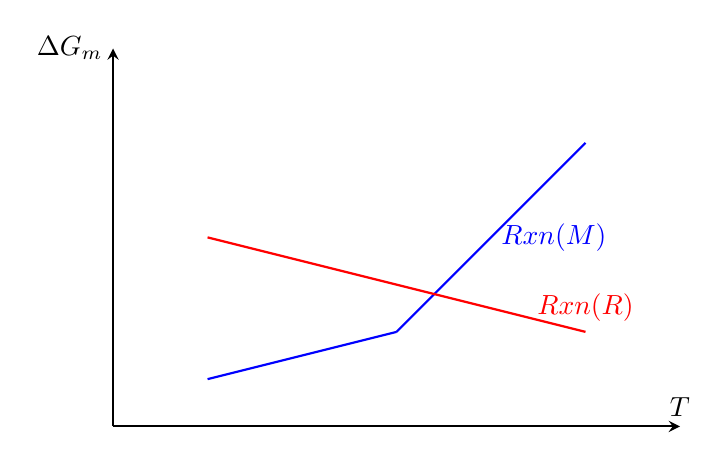
\begin{tikzpicture}[scale=1.2,
                    >=stealth,
                    axis/.style={thick,black}]

\draw[axis,->] (0,0) -- (6,0) node[above] {$T$}; 
\draw[axis,->] (0,0) -- (0,4) node[left] {$\Delta G_m$}; 

\draw[thick,blue] (1,0.5) -- (3,1) node[midway,above right]{};
\draw[thick,blue] (3,1) -- (5,3) node[midway,right] {$Rxn(\text{M})$};
\draw[thick,red] (1,2) -- (5,1) node[right,above] {$Rxn(\text{R})$};

\end{tikzpicture} 
\end{center}

其中斜率为$-\Delta_r S_m$，偏摩尔Gibbs自由能的零点为$T_0 = {\Delta_r H_m}/{\Delta_r S_m}$，其自发的转变温度，即偏摩尔Gibbs自由能小于0以下对应温度是自发的，而对一个耦合的反应，我们还是以金属冶炼为例，还原剂在金属线下是自发。

图中还有一个令人注意的点，即我们的金属线发生了转折，显然这源于熔化，减少了熵变，导致斜率提高。
\end{definition}

\newpage
